\documentclass[a4paper,12pt]{article}

\usepackage[spanish]{babel}
\usepackage[utf8]{inputenc}
\usepackage[T1]{fontenc}
\usepackage[utf8]{inputenc}
\usepackage{makeidx}
\usepackage{graphicx}
\usepackage{lmodern}
\usepackage{kpfonts}
\usepackage[left=2cm,right=2cm,top=2cm,bottom=2cm]{geometry}
\usepackage{amsmath,amsfonts,amssymb}
\usepackage{setspace}

\title{Parcial 2}
\author{Junior Miguel Lara Torres}
\date{today}

\graphicspath {{C:/Users/JuniorLara/Desktop/TexMaker_Files/}}
\begin{document}

\begin{center}
\par 
\includegraphics[scale=1]{USB} \par
Universidad Simon Bolivar \\ Curso: CI2613 / Algoritmos y Estructuras III \\ Trimestre: Septiembre-Diciembre, 2022 \\ Profesor: Wilmer Bandres \\ Estudiante: Junior Miguel Lara Torres - Carnet: 17-10303 \\
\end{center}

\begin{center}
Parcial 2
\end{center}

\textbf{ * Repaso de conceptos (8 pts)}

\begin{enumerate}

\item Marque las casillas de las proposiciones que sean verdaderas (4 pts).

Las proposiciones verdaderas son:
\begin{itemize}

\item En un árbol de DFS de un grafo dirigido existen arcos cruzados (cross-edges).

\item En un grafo conexo con costos en los arcos la existencia de un ciclo de costo negativo implica la inexistencia de caminos de costo mínimo hasta cada nodo.

\item En un grafo sin costos en los arcos, DFS puede ser usado para calcular el camino que usa la menor cantidad de arcos hasta cada nodo empezando desde un nodo fuente.

\item El algoritmo Bellman-Ford puede ser usado en un grafo con costos negativos y calcula caminos de costo mínimo o detecta ciclos negativos.

\item En el algoritmo de Kruskal cada nodo empieza siendo un árbol aislado.

\end{itemize}


\item Aplique Dijkstra en el siguiente grafo desde el nodo A. En cada paso indique que nodo es sacado del priority queue y finalmente indique el costo del camino de costo mínimo hasta cada nodo del grafo. (2 pts)
\begin{center}
\par 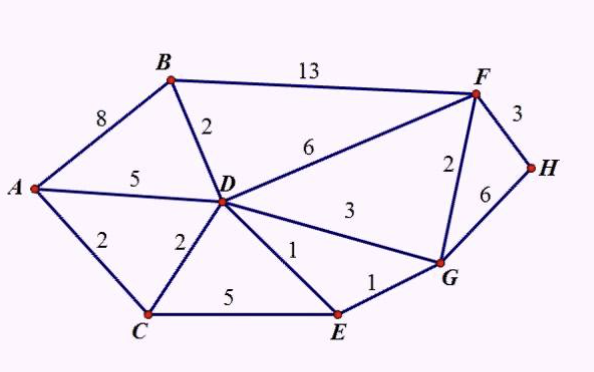
\includegraphics[scale=1.3]{grafosec1} \par
\end{center}

Paso 1: Sale nodo A con costo 0.

Paso 2: Sale nodo C con costo 2.

Paso 3: Sale nodo D con costo 4.

Paso 4: Sale nodo E con costo 5.

Paso 5: Sale nodo B con costo 6.

Paso 6: Sale nodo G con costo 6.

Paso 7: Sale nodo F con costo 8.

Paso 8: Sale nodo H con costo 11.

\item Aplique el algoritmo de Prim en el grafo de la pregunta anterior empezando desde el nodo A. En cada paso indique qué nodo se va uniendo al MST  y finalmente indique el costo del MST. (2 pts)

Inicialmente se tiene el nodo A en el M.S.T.

Paso 1: Se une el nodo C con key 2. \\
Paso 2: Se une el nodo D con key 2. \\
Paso 3: Se une el nodo E con key 1. \\
Paso 4: Se une el nodo G con key 1. \\
Paso 5: Se une el nodo B con key 2. \\
Paso 6: Se une el nodo F con key 2. \\
Paso 7: Se une el nodo H con key 3. \\

Finalmente, el M.S.T. tendrá costo 13.

\end{enumerate}

\textbf{ * Ejercicios (10 pts)}

\begin{enumerate}

\item Dado un grafo dirigido $G=(V,E)$, dos nodos $s$ y $t$,  y una función de costo sobre los arcos del grafo. Describa un algoritmo que funcione en tiempo $O(|V|^3)$ que calcule el camino de costo mínimo desde $s$ a $t$ que contenga por lo menos $|V|$ arcos. (5 pts).

\begin{itemize}

\item Algoritmo:

Se crea una subrutina de nombre RelajarInvert, recibe como argumentos de entrada dos nodos $x$ e $y$ y esta subtutina tiene acceso a los arreglos de distancias y arcos usados. Posee como condicional en caso de distancia de $y$ sea menor que la suma de la distancia de $x$ mas el costo del arco que une a $x$ e $y$, entonces la distancia de $y$ se le asigna dicha suma. Aumenta el numero de arcos usado para el nodo adyacente. En caso de encontrar que el nodo adyacente es igual al T y el numero de arcos usados para el nodo T es mayor o igual al número de nodos entonces retornamos True, de lo contrario siempre retornamos False.

Bool RelajarInvert( nodo x, nodo y ) $\{$ \\
$~~~~~~~~$ if $d[y] < d[x]+c(x,y)$ $\{$ \\
$~~~~~~~~~~~~~~~~$ $d[y] = d[x]+c(x,y)$; \\
$~~~~~~~~~~~~~~~~$ $arc-use[y]++$; \\
$~~~~~~~~~~~~~~~~$ if $ y == t \land arc-use[y] \geq |V|$ 	$\{$ \\	
$~~~~~~~~~~~~~~~~~~~~~~~~$ return $True$;\\
$~~~~~~~~~~~~~~~~$ $\{$ \\
$~~~~~~~~$ $\}$ \\
$~~~~~~~~$ return $False$; \\	
$\}$ \\

Aplicando una noción de Bellmand-Ford. Se tendrá inicialmente un arreglo de Distancias inicializado en menos infinito para cada nodo del grafo. También un arreglo de Arcos Usados inicializado en 0 para cada nodo del grafo.

Como se habla de grafo dirigido, entonces tomamos como nodo fuente a S.
Para el nodo fuente se marca en el arreglo de distancia en 0. Aplicamos un bucle por el número de nodos al cuadrado($|V|^2$). Este bucle tendrá a otro bucle interno por el número de arcos ($|E|$) y dentro de este bucle interno se realiza RelajarInvert para el arco en cuestión. Como RelajarInvert retorna un valor Bool, en caso de retornar False se sigue el proceso(este False simula el no haber completado el objetivo), en caso de retornar True entonces hemos dado con el camino de costo mínimo desde S hasta T, cuyo valor esta almacenado en la posición T del arreglo de distancias. 

Una vez finalicen los bucles anidados anteriores y la subrutina RelajarInvert no haber retornado True, entonces no hemos dado con el objetivo, por tanto no existe camino desde S hasta T.

BF-Update( Grafo G, Nodo Fuente S, Nodo Llegada T, función c ) $\{$\\
$~~~~~~~~$ $d[v] \leftarrow -\infty ~~ \forall v\in V$;\\
$~~~~~~~~$ $d[S] \leftarrow 0$;\\
$~~~~~~~~$ for $k = 1 \to |V|^2$ $\{$\\
$~~~~~~~~~~~~~~~~$ for $e=(x,y)\in E$ $\{$\\ 
$~~~~~~~~~~~~~~~~~~~~~~~~$ if $RelajarInvert(x,y)$ $\{$\\
$~~~~~~~~~~~~~~~~~~~~~~~~~~~~~~~~$ return $d[y]$;\\
$~~~~~~~~~~~~~~~~~~~~~~~~$ $\}$\\
$~~~~~~~~~~~~~~~~$ $\}$ \\
$~~~~~~~~$ $\}$\\
$~~~~~~~~$ return 'No camino S a T';\\
$\}$ \\

\item Análisis y Correctitud:

Como se tiene un grafo cuya condición establecida por el problema es que sea dirigido, entonces en primer lugar podemos asumir que el grado dado puede contener varias C.F.C., si se da el caso de S y T estar en distintas C.F.C. obtendremos que 'No camino S a T', pues no habrá arco que pueda ser relajado y que vaya formando un camino desde S a T ya que no existe un camino posible. 

Por otra parte, si se tiene que el grado exterior de S es 0, entonces no existe arco de salida por lo que no es posible formar un camino desde S hasta donde quiera que este T, de la misma forma si el grado interior de T es 0 entonces no existe arco de llagada. En estos casos la subrutina nunca encontrará el objetivo. 

Adicionalmente, como el camino de costo mínimo formado desde S hasta T puede tener mas de $|V|$ entonces debemos iterar en el peor de los casos $|V|^2$ veces para garantizar la suficiente relajación de los arcos y conseguir el camino desde S a T. Ahora, es importante destacar que se relaja aumentado los costos(RelajarInvert), básicamente hasta encontrar para el nodo destino T el costo mínimo, pues durante el camino puede ocurrir múltiples recorridos en ciclos de costo positivo hasta llegar al numero de arcos ($\geq |V|$) y una vez relajemos un arco que conecte con T y este tenga arcos usados $\geq |V|$ por primera vez, entonces hemos encontrado el camino de costo mínimo de S a T de por lo menos $|V|$ arcos. \\

\item Complejidad:

Veamos que se tiene como base una estructura similar a la del Algoritmo Bellmand-Ford, este cumple con complejidad $O(|V||E|)$, en este caso se tiene el bucle anidado con iteración hasta $]V]^2$ y luego sobre el número de arcos y como la subrutina es $O(1)$ decimos entonces que la complejidad de BF-Update es de $O(|V|^2|E|)$.

\end{itemize}

\item Dado un grafo no dirigido y conexo $G = (V,E)$ con exactamente $|V|$ arcos $(|V| = |E|)$ y una función de costo sobre los arcos, describa un algoritmo en tiempo $O(|V|)$ para determinar un camino de costo mínimo desde un nodo $s$ a un nodo $t$. (5pts)

\begin{itemize}

\item Algoritmo:

Se plantea la noción de Búsqueda en Amplitud(BFS)sobre grafos. Se tendrá inicialmente un arreglo de Distancias y una cola Q.

Tomamos bien sea S o T como nodo raíz. Agregamos a la cola el nodo raíz.
Para todos los nodos del grafo marcamos en infinito el vector de distancia, pero marcamos en 0 el nodo raíz. Hacemos push del elemento raíz en la cola. Realizamos un bucle mientras la cola no este vacía. 

Una vez en el bucle, ver el nodo front de la cola. Hacemos pop del front en cola. Realizamos un bucle por todos los arcos de salida del nodo popeado, este bucle tiene como condición revisar que si la distancia del adyacente es mayor que la distancia del nodo front mas el costo del arco que los une, entonces actualizamos la distancia del nodo adyacente con la suma de la distancia del nodo front mas el costo del arco que los une como también hacer push del nodo adyacente a la cola, de lo contrario proceder con el siguiente arco.

Una vez finalice el bucle interno sobre los arcos del nodo front, entonces comienza una nueva iteración del bucle principal cuya condición es mientras este vacía la cola. 

Al finalizar el bucle externo, vamos al arreglo de distancias y en la posición que corresponde al nodo T se encuentra el costo del camino mínimo desde S hasta T.

\item Análisis y Correctitud:

Este algoritmo mezcla las ideas de BFS con Dijkstra. Una vez estando en el bucle principal condicionado por el size de la cola, al tomar de la cola el front analizamos sobre este front todos los nodos adyacentes a él y como hablamos de grafo no dirigido contamos incluso a nodos ya procesados(que fueron retirados de la cola) pero asumiendo que la función de costo sobre los arcos asigna valores No negativos a los arcos entonces garantizamos la no existencia de ciclos de coste negativo dentro del grafo. 

Asi, en el bucle interno sobre los arcos obtenemos un condicional que actualiza cuando se encuentra un camino al nodo adyacente procesado en cuestión que es menor al que tiene y que se PUSHEA nuevamente, es decir cuando un nodo sale de la cola no necesariamente posee el costo menor ya calculado, pues si un nodo ya fue popeado y luego en un futuro este encuentra una menor distancia entonces lo pusheamos nuevamente a la cola para posteriores actualizaciones de nodos adyacentes. 

Por tanto, cuando termina el bucle principal si habíamos marcado como nodo raíz a S, debemos solamente buscar en el arreglo de distancia para el nodo T y este valor indica el costo mínimo del camino entre la S y T. \\

\item Complejidad:

Hemos aplicado un BFS ajustado al problema, con dichos ajustes no alteran de forma critica al algoritmo original seguimos teniendo la complejidad del BFS el cual es $O(|V|+|E|)$, pero como $(|V| = |E|)$ para este caso particular entonces tenemos $O(|V|+|V|)=O(2|V|)=O(|V|)$.

\end{itemize}

\end{enumerate}

\textbf{ * Demostraciones y contraejemplos (12 pts))}

\begin{enumerate}

\item Demuestre la subóptimalidad de un camino de costo mínimo, es decir que un subcamino de un camino óptimo entre dos nodos es también óptimo. (4 pts)

Partiendo de la idea de tener un camino optimo entre cualquier par de nodos $x$ e $y$ denotado $P:\langle x, ..., z,..., z', ... y \rangle$, por tanto tomando $z$ y $z'$, como nodos intermedios pertenecientes a P, formamos el camino $P': \langle z, ..., z' \rangle$ . Suponemos ahora que $P'$ no es óptimo, de esto obtenemos que el costo de $P'$ se denota como $c(P')$ y el costo del camino óptimo entre $z$ y $z'$ es $\delta_z(z')$ y sabemos que $\delta_z(z') < c(P')$ porque $P'$ no es óptimo. 

Adicionalmente, el camino óptimo entre $z$ y $z'$ es denotado por $O: \langle z,..., z' \rangle$. Entonces, si creamos un camino $P''$ tal que sea igual al $P$ menos $P'$ y agregando $O$, entonces el costo de $P''$ esta determinado por $c(P'') = c(P)-c(P')+\delta_z(z')$  y por fórmula anterior $-c(P')+\delta_z(z') < 0$ por tanto, este número es menor que cero y se reduce $c(P)$ lo que indica que $P''$ es un mejor camino que $P$ lo cual contradice el hecho de suponer $P$ óptimo.

Finalmente, decimos que todo sub-camino en un camino optimo también es óptimo.

\item Dé un contraejemplo de la siguiente proposición: Dijkstra calcula caminos de costo mínimo en un grafo no dirigido con costos negativos que no contiene ciclos de costo negativo (4 pts)

Se tiene el siguiente grafo
\begin{center}
\par 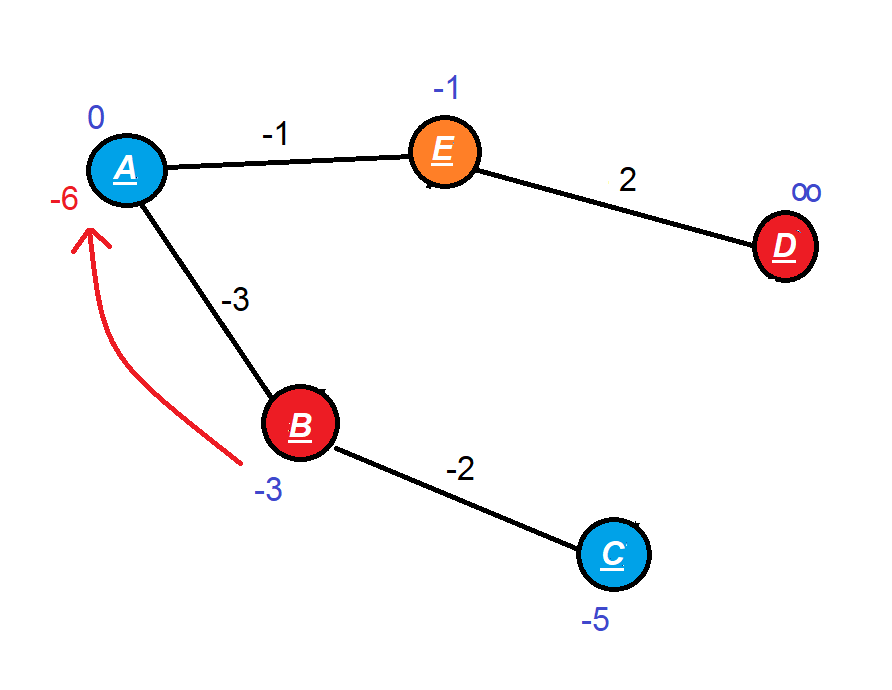
\includegraphics[scale=0.8]{g1p2} \par
\end{center}

En la implementacion establecida para Dijsktra cuyo paso de 'Relajación' esta determinada por $d[ady] > d[n]+c(\{n, ady\})$, con $d$ vector de distancias y $c$ función de costos sobre los arcos. Esta función c al asignar costos negativos ocasiona lo marcado por la fecha ROJA en el gráfico, el nodo A tenia costo 0, luego pasa a valor -6 debido a la condición de relajación $0 > -3 + -3$. Como por correctitud del Dijkstra, un nodo que sale de la cola tiene el costo mínimo calculado hasta la fuente, pero acabamos de notar que el nodo A(había salido de la cola) pasa de 0 a -6 lo cual contradice la correctitud del Dijkstra.

\item Demuestre o dé un contraejemplo: Dado un grafo no dirigido y sin costos en los arcos y un nodo fuente s, BFS puede ser usado para calcular caminos con la mínima cantidad de arcos desde s hasta cada nodo del grafo (4pts)

Sabemos que por BFS se tiene un vector/estructura de datos que permite almacenar el "nivel" del nodo en que fueron procesados en el método BFS. Dicha información contiene para el nodo raíz($s$) nivel 0 como base, luego todo nodo adyacente al $s$ tendrá nivel 0 + 1 debido al for interno del BFS, esto dice que todo nodo adyacente usa nivel 0 + 1 arcos como mínimo y el nodo $s$ usa nivel 0 arcos.

En un análisis posterior, podemos obtener un arco que conecta un nodo con un adyacente ya procesado, es decir un nivel será actualizado en nivel(ady) = nivel(nodo) + 1 si este esta en -1(Indicando que no ha sido procesado) de lo contrario estamos procesando un adyacente que esta en el mismo nivel que el nodo o incluso inferior. 

Asimismo, aplicando una noción inductiva, tenemos que un nodo k tiene nivel x y usa x arcos desde la fuente, cualquier nodo adyacente no procesado tendrá nivel x + 1 y usa x+1 arcos como mínimo desde la fuente.

Finalmente, BFS permite determinar los caminos mas cortos desde un nodo fuente a cualquier otro nodo del grafo mediante los niveles formados en el recorrido BFS.

\end{enumerate}

\end{document}